\section{Addition by a Known Classical Value}
\label{sec:addition}

Adding a (known) classical integer ($m$) to a quantum register encoded in binary is a required operation throughout this work:
\begin{equation}
    \label{eq:addition-by-classical-value}
    \ket{n} \rightarrow \ket{n + m}
\end{equation}
In an effort to keep this work self-contained and pedagogical, we review some methods for constructing this operation in this section.

\begin{figure}
    \centering
    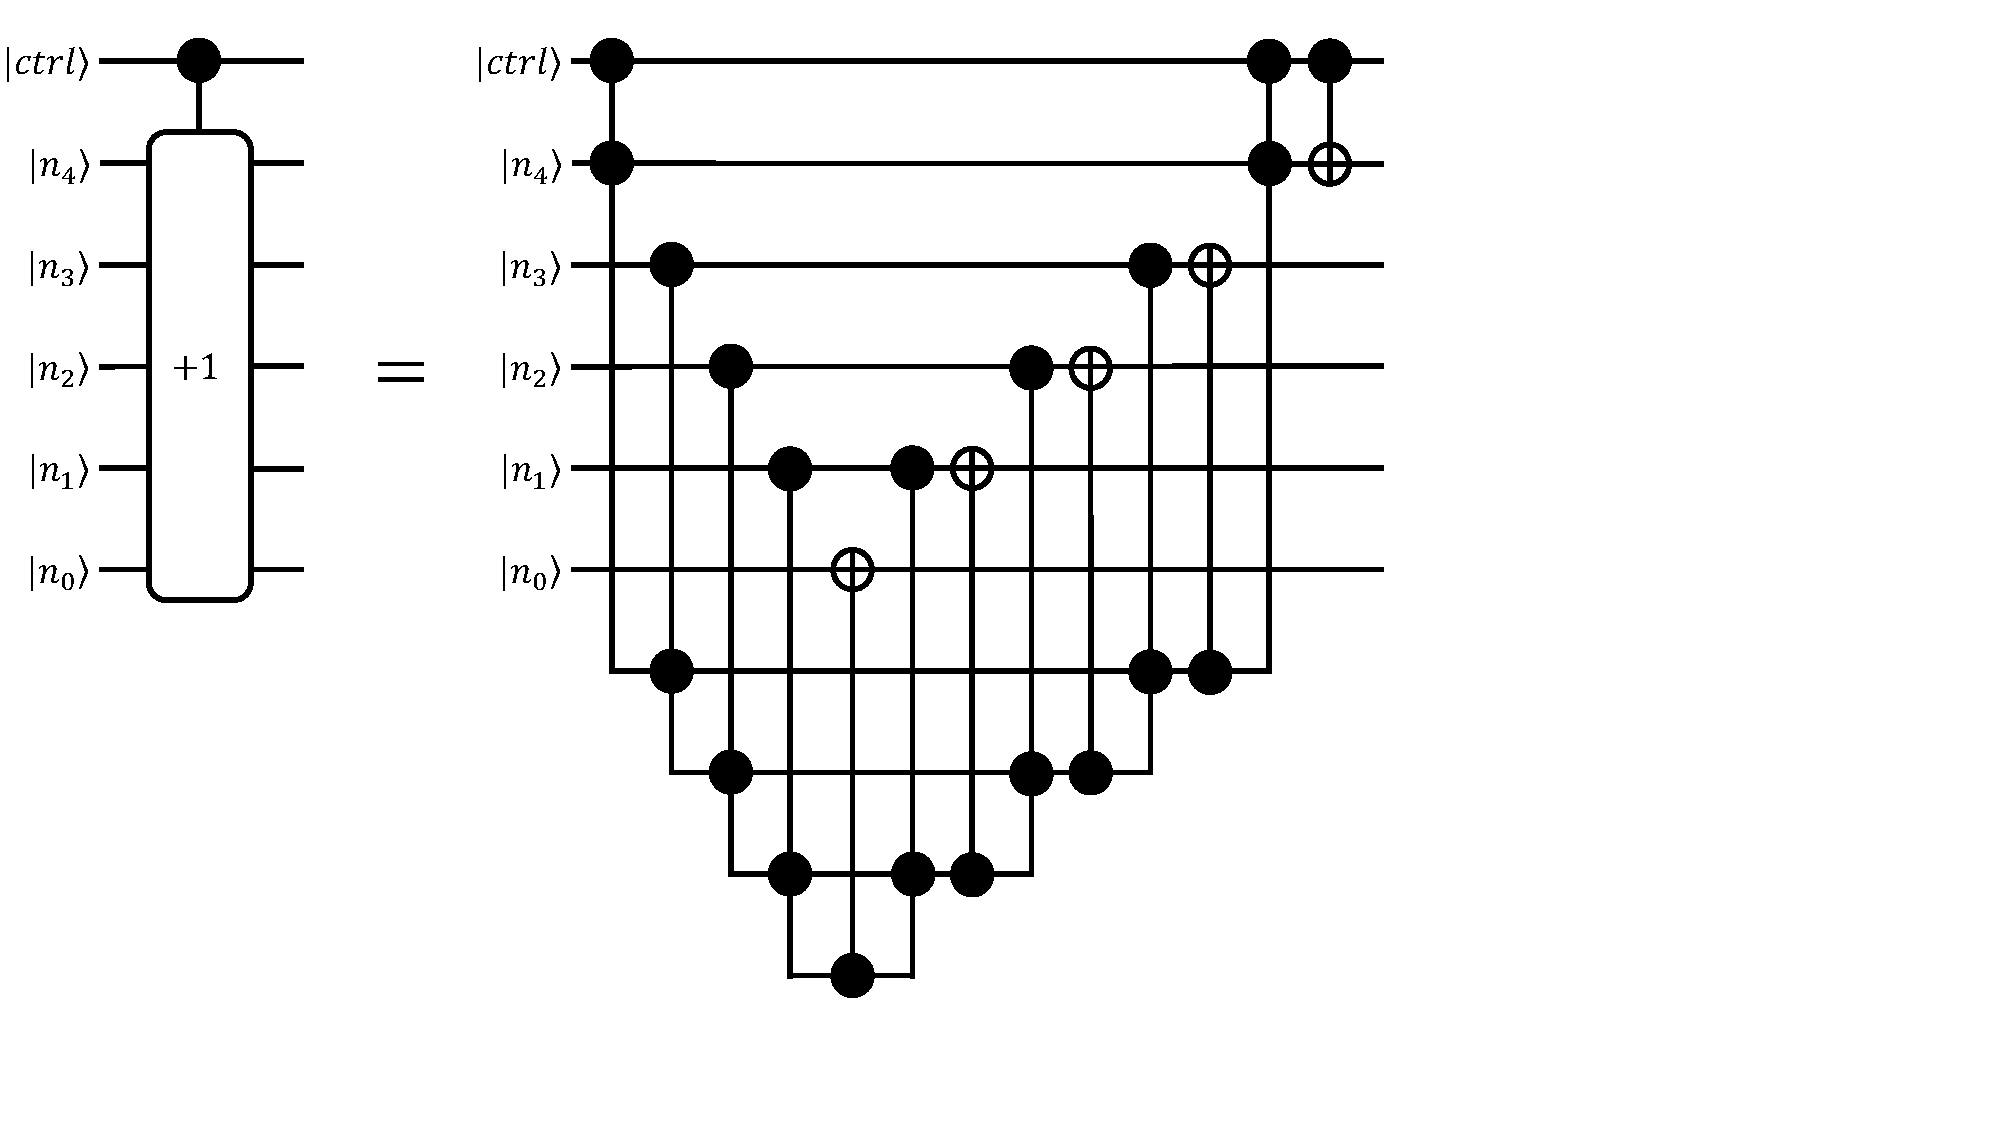
\includegraphics[width=8cm]{figures/incrementer.pdf}
    \caption{
        \textbf{Controlled Incrementer} 
        A circuit diagram implementing a controlled incrementer (mod $32$) is shown.
        The controlled incrementer performs the operation $\ket{x} \rightarrow \ket{x + 1}$ when the control qubit is in the $\ket{1}$ state.
        Decrementing the register by $1$ can be achieved by applying Pauli-X gates on each qubit before and after the operation.
    }
    \label{fig:incrementer}
\end{figure}


One option is to use a series of controlled incrementer ($+1$) circuits.
An implementation of an incrementer circuit given by Gideny \cite{Gidney_2015} is shown in Figure \ref{fig:incrementer}.
If $N$ is the number of qubits in the register being incremented, this implementation requires $4(N-1)$ T gates and $N-1$ clean ancillae.
Naively, a series of $m$ incrementers will result in increasing the value of the register by $m \mod 2^N$.

\begin{figure}
    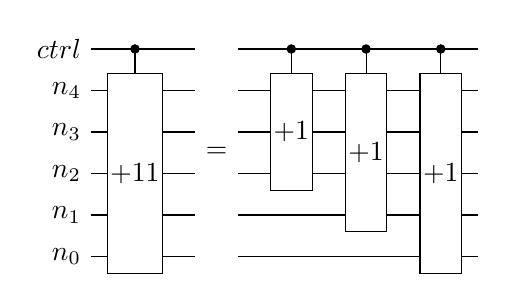
\begin{tikzpicture}[scale=1.000000,x=1pt,y=1pt]
\filldraw[color=white] (0.000000, -7.500000) rectangle (140.000000, 82.500000);
% Drawing wires
% Line 1: ctrl W ctrl
\draw[color=black] (0.000000,75.000000) -- (140.000000,75.000000);
\draw[color=black] (0.000000,75.000000) node[left] {$ctrl$};
% Line 2: n4 W n_4
\draw[color=black] (0.000000,60.000000) -- (140.000000,60.000000);
\draw[color=black] (0.000000,60.000000) node[left] {$n_4$};
% Line 3: n3 W n_3
\draw[color=black] (0.000000,45.000000) -- (140.000000,45.000000);
\draw[color=black] (0.000000,45.000000) node[left] {$n_3$};
% Line 4: n2 W n_2
\draw[color=black] (0.000000,30.000000) -- (140.000000,30.000000);
\draw[color=black] (0.000000,30.000000) node[left] {$n_2$};
% Line 5: n1 W n_1
\draw[color=black] (0.000000,15.000000) -- (140.000000,15.000000);
\draw[color=black] (0.000000,15.000000) node[left] {$n_1$};
% Line 6: n0 W n_0
\draw[color=black] (0.000000,0.000000) -- (140.000000,0.000000);
\draw[color=black] (0.000000,0.000000) node[left] {$n_0$};
% Done with wires; drawing gates
% Line 8: n4 n3 n2 n1 n0 G width=20 $+11$ ctrl
\draw (16.000000,75.000000) -- (16.000000,0.000000);
\begin{scope}
\draw[fill=white] (16.000000, 30.000000) +(-45.000000:14.142136pt and 50.911688pt) -- +(45.000000:14.142136pt and 50.911688pt) -- +(135.000000:14.142136pt and 50.911688pt) -- +(225.000000:14.142136pt and 50.911688pt) -- cycle;
\clip (16.000000, 30.000000) +(-45.000000:14.142136pt and 50.911688pt) -- +(45.000000:14.142136pt and 50.911688pt) -- +(135.000000:14.142136pt and 50.911688pt) -- +(225.000000:14.142136pt and 50.911688pt) -- cycle;
\draw (16.000000, 30.000000) node {$+11$};
\end{scope}
\filldraw (16.000000, 75.000000) circle(1.500000pt);
% Line 10: =
\draw[fill=white,color=white] (38.000000, -6.000000) rectangle (53.000000, 81.000000);
\draw (45.500000, 37.500000) node {$=$};
% Line 12: n4 n3 n2 G width=15 $+1$ ctrl
\draw (72.500000,75.000000) -- (72.500000,30.000000);
\begin{scope}
\draw[fill=white] (72.500000, 45.000000) +(-45.000000:10.606602pt and 29.698485pt) -- +(45.000000:10.606602pt and 29.698485pt) -- +(135.000000:10.606602pt and 29.698485pt) -- +(225.000000:10.606602pt and 29.698485pt) -- cycle;
\clip (72.500000, 45.000000) +(-45.000000:10.606602pt and 29.698485pt) -- +(45.000000:10.606602pt and 29.698485pt) -- +(135.000000:10.606602pt and 29.698485pt) -- +(225.000000:10.606602pt and 29.698485pt) -- cycle;
\draw (72.500000, 45.000000) node {$+1$};
\end{scope}
\filldraw (72.500000, 75.000000) circle(1.500000pt);
% Line 13: n4 n3 n2 n1 G width=15 $+1$ ctrl
\draw (99.500000,75.000000) -- (99.500000,15.000000);
\begin{scope}
\draw[fill=white] (99.500000, 37.500000) +(-45.000000:10.606602pt and 40.305087pt) -- +(45.000000:10.606602pt and 40.305087pt) -- +(135.000000:10.606602pt and 40.305087pt) -- +(225.000000:10.606602pt and 40.305087pt) -- cycle;
\clip (99.500000, 37.500000) +(-45.000000:10.606602pt and 40.305087pt) -- +(45.000000:10.606602pt and 40.305087pt) -- +(135.000000:10.606602pt and 40.305087pt) -- +(225.000000:10.606602pt and 40.305087pt) -- cycle;
\draw (99.500000, 37.500000) node {$+1$};
\end{scope}
\filldraw (99.500000, 75.000000) circle(1.500000pt);
% Line 14: n4 n3 n2 n1 n0 G width=15 $+1$ ctrl
\draw (126.500000,75.000000) -- (126.500000,0.000000);
\begin{scope}
\draw[fill=white] (126.500000, 30.000000) +(-45.000000:10.606602pt and 50.911688pt) -- +(45.000000:10.606602pt and 50.911688pt) -- +(135.000000:10.606602pt and 50.911688pt) -- +(225.000000:10.606602pt and 50.911688pt) -- cycle;
\clip (126.500000, 30.000000) +(-45.000000:10.606602pt and 50.911688pt) -- +(45.000000:10.606602pt and 50.911688pt) -- +(135.000000:10.606602pt and 50.911688pt) -- +(225.000000:10.606602pt and 50.911688pt) -- cycle;
\draw (126.500000, 30.000000) node {$+1$};
\end{scope}
\filldraw (126.500000, 75.000000) circle(1.500000pt);
% Done with gates; drawing ending labels
% Done with ending labels; drawing cut lines and comments
% Done with comments
\end{tikzpicture}

    \caption{
        \textbf{Addition via Incrementers} 
        An implementation of addition by a classical value ($11$) (mod $32$) using a series of incrementers is shown.
        An incrementer applied onto a register excluding the least-significant qubit implements a bit-shifted incrementer.
        This effectively increases the value of the register by $2$.
        Addition by the classical value $11$ can be constructed by bit-shifted incrementers adding the values $+8$, $+2$, and $+1$.
        Subtraction by the same value can be achieved by applying Pauli-X gates on each qubit before and after the operation.
    }
    \label{fig:addition-via-incrementers}
\end{figure}


However, an incrementer circuit can also be used to perform addition by a power of $2$ by acting on only the most-significant qubits.
For example, adding the value $8$ can be achieved using an incrementer circuit that treats the $4^{th}$ least significant qubit as the least significant qubit in the incrementer circuit and disregards the $3$ lesser qubits.
A circuit adding any classical value can then be constructed based on the binary representation of the classical number.
A circuit diagram for this construction is shown in Figure \ref{fig:addition-via-incrementers}.
The cost of this construction would require $N$ incrementer circuits requiring $4 \sum_{i=0}^{N - 2} N - i - 1$ T gates in total and $N - 1$ clean ancillae.

Since we are performing modular addition, the same result can also be achieved by subtracting the value $2^N - m$.
As an example, if the classical value is $31$ and $N = 5$, then this can be accomplished using a single decrementer circuit which can be constructed by conjugating an incrementer circuit with Pauli X gates acting on the qubits encoding $\ket{n}$.
The cost of these two methods can be classically determined and the more favorable option can be chosen during compilation.
The upper bound for the number of T gates, regardless of the classical value being added, is $N^2 + N$.
\ws{This scaling was determined numerically, but i think it shouldn't be hard to derive.}


\begin{figure}
    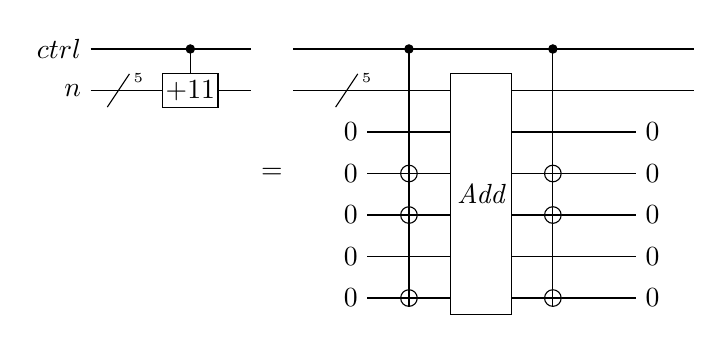
\begin{tikzpicture}[scale=1.000000,x=1pt,y=1pt]
\filldraw[color=white] (0.000000, -7.500000) rectangle (218.000000, 97.500000);
% Drawing wires
% Line 1: ctrl W ctrl
\draw[color=black] (0.000000,90.000000) -- (218.000000,90.000000);
\draw[color=black] (0.000000,90.000000) node[left] {$ctrl$};
% Line 2: n W n
\draw[color=black] (0.000000,75.000000) -- (218.000000,75.000000);
\draw[color=black] (0.000000,75.000000) node[left] {$n$};
% Line 3: m4 W 0 0
\draw[color=black] (92.500000,60.000000) -- (204.500000,60.000000);
% Line 4: m3 W 0 0
\draw[color=black] (92.500000,45.000000) -- (204.500000,45.000000);
% Line 5: m2 W 0 0
\draw[color=black] (92.500000,30.000000) -- (204.500000,30.000000);
% Line 6: m1 W 0 0
\draw[color=black] (92.500000,15.000000) -- (204.500000,15.000000);
% Line 7: m0 W 0 0
\draw[color=black] (92.500000,0.000000) -- (204.500000,0.000000);
% Done with wires; drawing gates
% Line 9: n / ^5
\draw (6.000000, 69.000000) -- (14.000000, 81.000000);
\draw (12.000000, 78.000000) node[right] {$\scriptstyle{^5}$};
% Line 11: n G width=20 $+11$ ctrl
\draw (36.000000,90.000000) -- (36.000000,75.000000);
\begin{scope}
\draw[fill=white] (36.000000, 75.000000) +(-45.000000:14.142136pt and 8.485281pt) -- +(45.000000:14.142136pt and 8.485281pt) -- +(135.000000:14.142136pt and 8.485281pt) -- +(225.000000:14.142136pt and 8.485281pt) -- cycle;
\clip (36.000000, 75.000000) +(-45.000000:14.142136pt and 8.485281pt) -- +(45.000000:14.142136pt and 8.485281pt) -- +(135.000000:14.142136pt and 8.485281pt) -- +(225.000000:14.142136pt and 8.485281pt) -- cycle;
\draw (36.000000, 75.000000) node {$+11$};
\end{scope}
\filldraw (36.000000, 90.000000) circle(1.500000pt);
% Line 13: =
\draw[fill=white,color=white] (58.000000, -6.000000) rectangle (73.000000, 96.000000);
\draw (65.500000, 45.000000) node {$=$};
% Line 15: n / ^5
\draw (88.500000, 69.000000) -- (96.500000, 81.000000);
\draw (94.500000, 78.000000) node[right] {$\scriptstyle{^5}$};
% Line 17: m4 START
\draw[color=black] (100.000000,60.000000) node[fill=white,left,minimum height=15.000000pt,minimum width=15.000000pt,inner sep=0pt] {\phantom{$0$}};
\draw[color=black] (100.000000,60.000000) node[left] {$0$};
% Line 18: m3 START
\draw[color=black] (100.000000,45.000000) node[fill=white,left,minimum height=15.000000pt,minimum width=15.000000pt,inner sep=0pt] {\phantom{$0$}};
\draw[color=black] (100.000000,45.000000) node[left] {$0$};
% Line 19: m2 START
\draw[color=black] (100.000000,30.000000) node[fill=white,left,minimum height=15.000000pt,minimum width=15.000000pt,inner sep=0pt] {\phantom{$0$}};
\draw[color=black] (100.000000,30.000000) node[left] {$0$};
% Line 20: m1 START
\draw[color=black] (100.000000,15.000000) node[fill=white,left,minimum height=15.000000pt,minimum width=15.000000pt,inner sep=0pt] {\phantom{$0$}};
\draw[color=black] (100.000000,15.000000) node[left] {$0$};
% Line 21: m0 START
\draw[color=black] (100.000000,0.000000) node[fill=white,left,minimum height=15.000000pt,minimum width=15.000000pt,inner sep=0pt] {\phantom{$0$}};
\draw[color=black] (100.000000,0.000000) node[left] {$0$};
% Line 22: ctrl +m3 +m2 +m0
\draw (115.000000,90.000000) -- (115.000000,0.000000);
\filldraw (115.000000, 90.000000) circle(1.500000pt);
\begin{scope}
\draw[fill=white] (115.000000, 45.000000) circle(3.000000pt);
\clip (115.000000, 45.000000) circle(3.000000pt);
\draw (112.000000, 45.000000) -- (118.000000, 45.000000);
\draw (115.000000, 42.000000) -- (115.000000, 48.000000);
\end{scope}
\begin{scope}
\draw[fill=white] (115.000000, 30.000000) circle(3.000000pt);
\clip (115.000000, 30.000000) circle(3.000000pt);
\draw (112.000000, 30.000000) -- (118.000000, 30.000000);
\draw (115.000000, 27.000000) -- (115.000000, 33.000000);
\end{scope}
\begin{scope}
\draw[fill=white] (115.000000, 0.000000) circle(3.000000pt);
\clip (115.000000, 0.000000) circle(3.000000pt);
\draw (112.000000, 0.000000) -- (118.000000, 0.000000);
\draw (115.000000, -3.000000) -- (115.000000, 3.000000);
\end{scope}
% Line 23: n m4 m3 m2 m1 m0 G width=22 $\textit{Add}$
\draw (141.000000,75.000000) -- (141.000000,0.000000);
\begin{scope}
\draw[fill=white] (141.000000, 37.500000) +(-45.000000:15.556349pt and 61.518290pt) -- +(45.000000:15.556349pt and 61.518290pt) -- +(135.000000:15.556349pt and 61.518290pt) -- +(225.000000:15.556349pt and 61.518290pt) -- cycle;
\clip (141.000000, 37.500000) +(-45.000000:15.556349pt and 61.518290pt) -- +(45.000000:15.556349pt and 61.518290pt) -- +(135.000000:15.556349pt and 61.518290pt) -- +(225.000000:15.556349pt and 61.518290pt) -- cycle;
\draw (141.000000, 37.500000) node {$\textit{Add}$};
\end{scope}
% Line 24: ctrl +m3 +m2 +m0
\draw (167.000000,90.000000) -- (167.000000,0.000000);
\filldraw (167.000000, 90.000000) circle(1.500000pt);
\begin{scope}
\draw[fill=white] (167.000000, 45.000000) circle(3.000000pt);
\clip (167.000000, 45.000000) circle(3.000000pt);
\draw (164.000000, 45.000000) -- (170.000000, 45.000000);
\draw (167.000000, 42.000000) -- (167.000000, 48.000000);
\end{scope}
\begin{scope}
\draw[fill=white] (167.000000, 30.000000) circle(3.000000pt);
\clip (167.000000, 30.000000) circle(3.000000pt);
\draw (164.000000, 30.000000) -- (170.000000, 30.000000);
\draw (167.000000, 27.000000) -- (167.000000, 33.000000);
\end{scope}
\begin{scope}
\draw[fill=white] (167.000000, 0.000000) circle(3.000000pt);
\clip (167.000000, 0.000000) circle(3.000000pt);
\draw (164.000000, 0.000000) -- (170.000000, 0.000000);
\draw (167.000000, -3.000000) -- (167.000000, 3.000000);
\end{scope}
% Line 25: m4 LABEL
% Line 26: m4 END
\draw[color=black] (197.000000,60.000000) node[fill=white,right,minimum height=15.000000pt,minimum width=15.000000pt,inner sep=0pt] {\phantom{$0$}};
\draw[color=black] (197.000000,60.000000) node[right] {$0$};
% Line 27: m3 END
\draw[color=black] (197.000000,45.000000) node[fill=white,right,minimum height=15.000000pt,minimum width=15.000000pt,inner sep=0pt] {\phantom{$0$}};
\draw[color=black] (197.000000,45.000000) node[right] {$0$};
% Line 28: m2 END
\draw[color=black] (197.000000,30.000000) node[fill=white,right,minimum height=15.000000pt,minimum width=15.000000pt,inner sep=0pt] {\phantom{$0$}};
\draw[color=black] (197.000000,30.000000) node[right] {$0$};
% Line 29: m1 END
\draw[color=black] (197.000000,15.000000) node[fill=white,right,minimum height=15.000000pt,minimum width=15.000000pt,inner sep=0pt] {\phantom{$0$}};
\draw[color=black] (197.000000,15.000000) node[right] {$0$};
% Line 30: m0 END
\draw[color=black] (197.000000,0.000000) node[fill=white,right,minimum height=15.000000pt,minimum width=15.000000pt,inner sep=0pt] {\phantom{$0$}};
\draw[color=black] (197.000000,0.000000) node[right] {$0$};
% Done with gates; drawing ending labels
% Done with ending labels; drawing cut lines and comments
% Done with comments
\end{tikzpicture}

    \caption{
        \textbf{Time-Efficient Controlled Addition of $11$}
        Increasing the value of a quantum register by a known classical value can be implemented using clean ancillae and an uncontrolled quantum addition circuit.
        The known classical value is loaded into a clean ancilla register using a series of CNOT gates corresponding to the binary representation of the classical value.
        Then an uncontrolled quantum addition circuit is applied to the two registers.
        Finally, the loading of the classical value is uncomputed.
    }
    \label{fig:addition-gate-efficient}
\end{figure}

Another option is to first load the classical value into an clean ancilla register, controlled on the control qubit, perform \textit{uncontrolled} (modular) addition of the two quantum registers, then ``unload'' the classical value.
If the control is off, then the classical value is not loaded and the uncontrolled addition simply adds the value $0$ and leaves the original register unchanged.
An example diagram for this construction depicting adding the value $m = 11$ to a register with $N = 5$ qubits is shown in Figure \ref{fig:addition-gate-efficient}.

The loading (and unloading) of the classical value only requires CNOTs and therefore does not contribute any non-Clifford resouces, but it does require $N$ clean ancillae.
However, if the $p$ least significant bits of $m$ are zero, then only $N - p$ qubits are required to load $m$ and the $p$ least-significant qubits of $N$ can be omitted from the addition.
Uncontrolled addition of two registers can be performed using $4(N-1)$ T gates and $N - 1$ clean ancillae using the construction for addition shown in Figure 1 of \cite{gidney2018halving}.
Therefore, in total, this compilation will require $4(N - p - 1)$ T gates and $2(N - p) - 1$ clean ancillae.

When $m$ is a power of $2$, then compilation using incrementer circuits uses the same number of T gates, but fewer clean ancillae.
When $m$ is not a power of $2$, then the compilation using uncontrolled quantum addition uses fewer T gates (at the expense of more clean ancillae).
Since $m$ is known during compilation, an implementation can be chosen that results in the fewest required resources.

\begin{figure*}
    \centering
    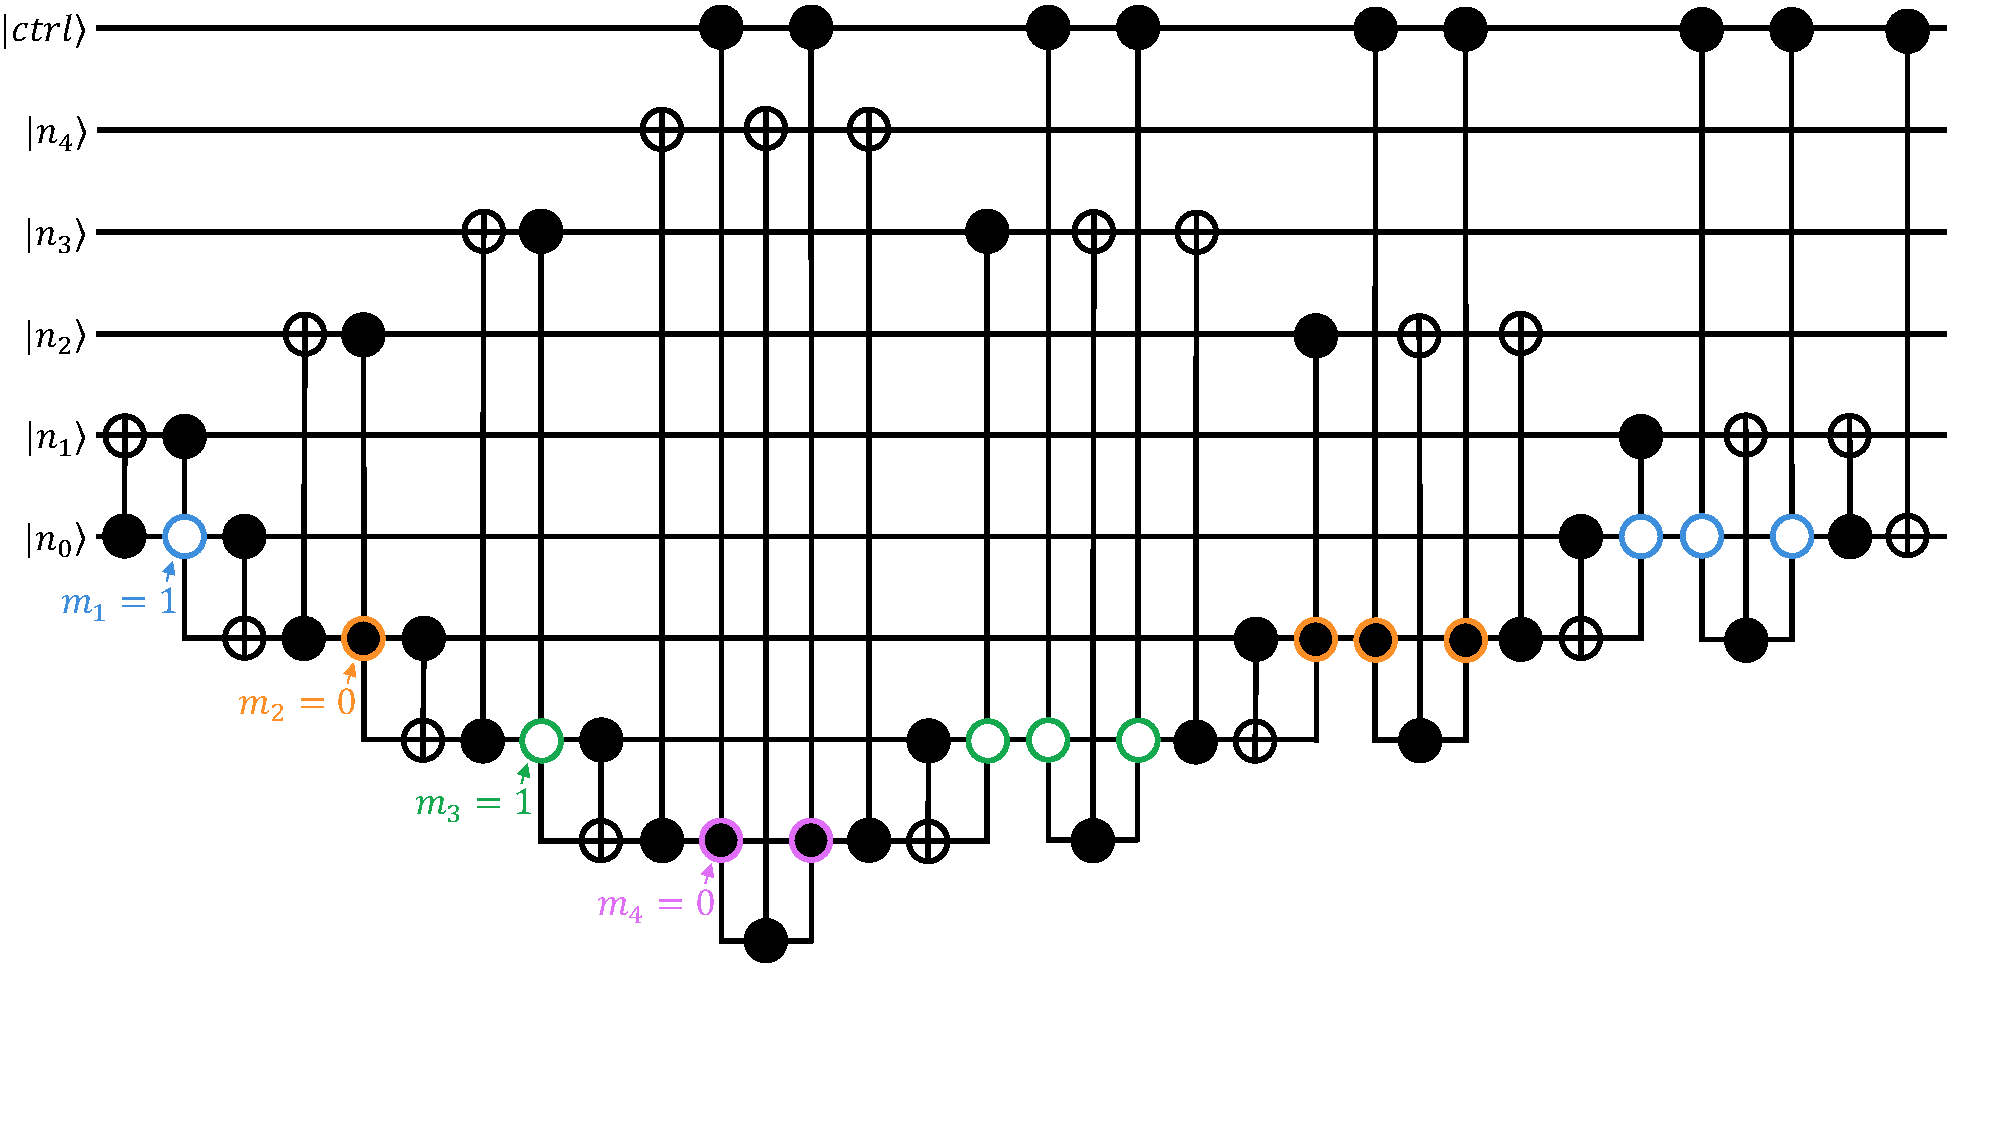
\includegraphics[width=12cm]{figures/ctrl-add-11-qubit-efficient.pdf}
    \caption{
        \textbf{Space-Efficient Controlled Addition of 11}
        An implementation for increasing the value of a register by a known classical value is shown for the case when the known value is $11$ and the number of qubits in the register is $5$.
        The binary representation of $11$ is $01011$ with the left-most bit being the most-significant.
        The values of these $M$ classical bits can be propagated into the control structure of the controlled quantum addition.
        If the value of the $i^\text{th}$ bit of $M$ is $0$ ($1$), the corresponding control in the circuit is controlled on the $\ket{1}$  ($\ket{0}$) state.
    }
    \label{fig:addition-qubit-efficient-11}
\end{figure*}

\begin{figure}
    \centering
    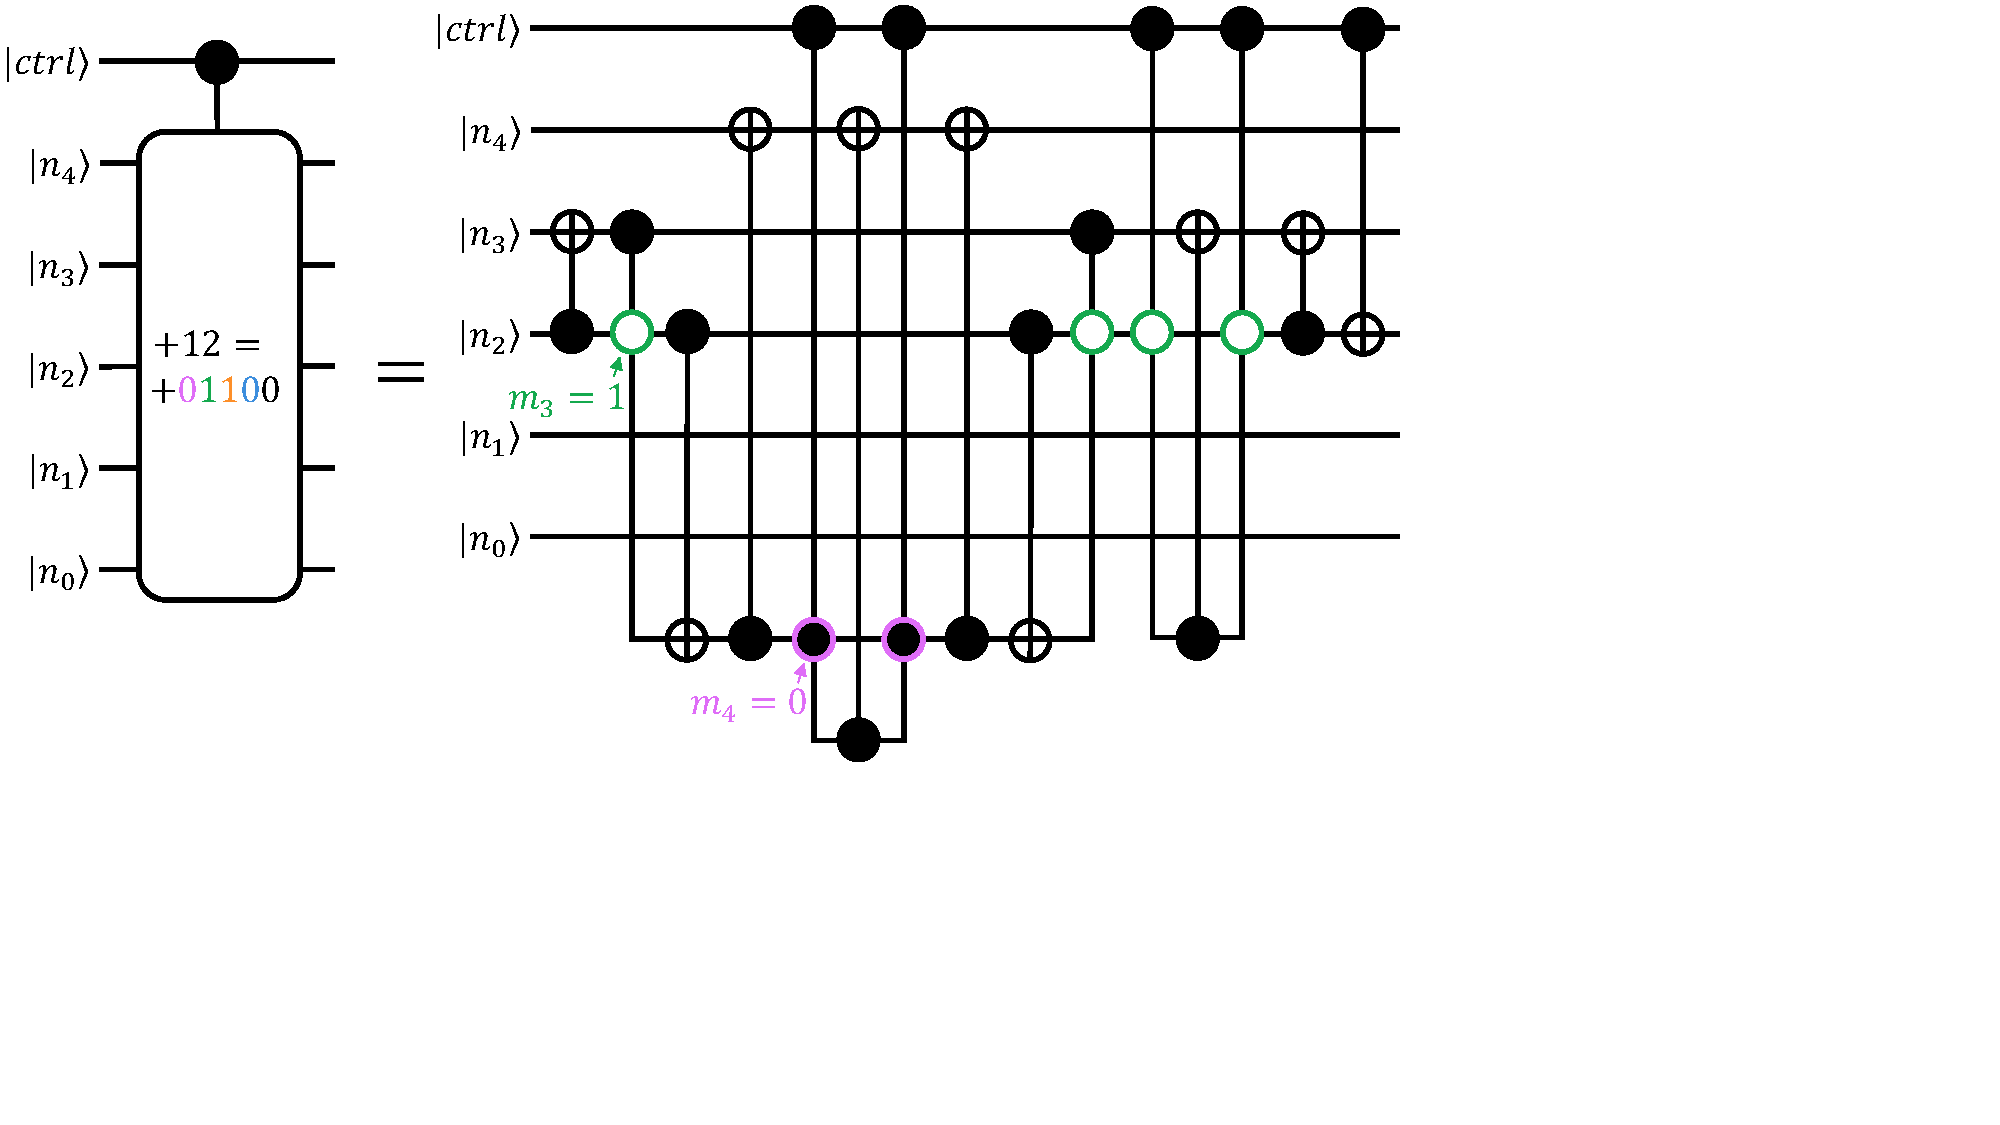
\includegraphics[width=8cm]{figures/ctrl-add-12-qubit-efficient.pdf}
    \caption{
        \textbf{Space-Efficient Controlled Addition of 12} 
        An implementation for increasing the value of a register by a known classical value is shown for the case when the known value is $12$ ($01100$ in binary) and the number of qubits in the register is $5$.
        When the least-significant bits of $M$ are $0$, the circuit can be bit-shifted, resulting in a lower cost implementation.
        In this case, the two least-significant bits are $0$, so the circuit can be bit-shifted twice.
    }
    \label{fig:addition-qubit-efficient-12}
\end{figure}

Another implementation can be chosen to reduce the number of clean ancillae, which uses the classical information about $m$ to modify the circuit for \textit{controlled} quantum addition.
Controlled addition of two registers can be performed using $4(2N - 3)$ T gates and $2N - 1$ clean ancillae using the construction for addition shown in Figure 4 of \cite{gidney2018halving}.
This circuit can be modified by propagating the classical information about the binary encoding of $m$ into the control structure of the adder circuit, thereby reducing the number of clean ancillae by $N$.
An example diagram showing this propagation in the case where $m = 11$ and $N = 5$ is shown in Figure \ref{fig:addition-qubit-efficient-11}.

Similarly, if the $p$ least-significant bits of $m$ are known to be zero, the addition can be performed beginning with the first non-zero bit of $m$.
An example circuit diagram for the case where $m=12$ ($01100$ in binary) and $N = 5$ is shown in Figure \ref{fig:addition-qubit-efficient-12}.
If the $p$ least significant bits of $m$ are zero, then this circuit uses $4(2(N - p) - 3)$ T gates and $N - p - 1$ clean ancillae.
Since this work primarily focuses on reducing the number of T gates, the quantum resource estimates quoted in this work do not utilize this strategy.
